\documentclass{article}


% if you need to pass options to natbib, use, e.g.:
%     \PassOptionsToPackage{numbers, compress}{natbib}
% before loading neurips_2022


% ready for submission
\usepackage{neurips_2022}


% to compile a preprint version, e.g., for submission to arXiv, add add the
% [preprint] option:
%     \usepackage[preprint]{neurips_2022}


% to compile a camera-ready version, add the [final] option, e.g.:
%     \usepackage[final]{neurips_2022}


% to avoid loading the natbib package, add option nonatbib:
%    \usepackage[nonatbib]{neurips_2022}


\usepackage[utf8]{inputenc} % allow utf-8 input
\usepackage[T1]{fontenc}    % use 8-bit T1 fonts
\usepackage{hyperref}       % hyperlinks
\usepackage{url}            % simple URL typesetting
\usepackage{booktabs}       % professional-quality tables
\usepackage{amsfonts}       % blackboard math symbols
\usepackage{nicefrac}       % compact symbols for 1/2, etc.
\usepackage{microtype}      % microtypography
\usepackage{xcolor}         % colors

\usepackage{pgfplots}
\usepackage{pgfplotstable}
\usepackage{subcaption}
\usepackage{tikz}
\usepackage{mathtools}
\usepackage{amsmath}


\pgfplotsset{compat=1.17}

\title{Formatting Instructions For NeurIPS 2022}


% The \author macro works with any number of authors. There are two commands
% used to separate the names and addresses of multiple authors: \And and \AND.
%
% Using \And between authors leaves it to LaTeX to determine where to break the
% lines. Using \AND forces a line break at that point. So, if LaTeX puts 3 of 4
% authors names on the first line, and the last on the second line, try using
% \AND instead of \And before the third author name.


\author{%
    David S.~Hippocampus\thanks{Use footnote for providing further information
    about author (webpage, alternative address)---\emph{not} for acknowledging
    funding agencies.} \\
    Department of Computer Science\\
    Cranberry-Lemon University\\
    Pittsburgh, PA 15213 \\
    \texttt{hippo@cs.cranberry-lemon.edu} \\
% examples of more authors
% \And
% Coauthor \\
% Affiliation \\
% Address \\
% \texttt{email} \\
% \AND
% Coauthor \\
% Affiliation \\
% Address \\
% \texttt{email} \\
% \And
% Coauthor \\
% Affiliation \\
% Address \\
% \texttt{email} \\
% \And
% Coauthor \\
% Affiliation \\
% Address \\
% \texttt{email} \\
}


\begin{document}


    \maketitle


    \begin{abstract}
        The abstract paragraph should be indented \nicefrac{1}{2}~inch (3~picas) on
        both the left- and right-hand margins. Use 10~point type, with a vertical
        spacing (leading) of 11~points. The word \textbf{Abstract} must be centered,
        bold, and in point size 12. Two line spaces precede the abstract. The abstract
        must be limited to one paragraph.
    \end{abstract}


    \section{Introduction}
    Recent advancements in large-scale pretrained networks, such as CLIP [1] or MAE [2], have demonstrated remarkable and generalizable performance across a variety of computer vision tasks. Conventionally, these networks are fine-tuned for specific downstream tasks by adjusting their weights through gradient descent, either by training an additional layer on top of the pretrained network or by fine-tuning the entire network. One limitation of this approach is that it necessitates a full copy of the fine-tuned weights to be stored for each downstream task, leading to significant memory requirements.

    In this work, we investigate the potential of identifying task-specific subnetworks that achieve good performance on downstream tasks, without modifying the original pretrained network weights. This approach can be implemented in a self-supervised or supervised manner and involves training a mask that selectively deactivates certain network weights. The mask is trained separately for each downstream task, enabling the network to dynamically adapt to different tasks.

    Moreover, this method can provide practical advantages in some scenarios, such as reducing memory requirements compared to standard fine-tuning techniques, as masks are smaller in size than full copies of the network weights. In this work, we examine the feasibility and effectiveness of this approach by evaluating it across various vision tasks and comparing it with standard fine-tuning methods.


    \subsection{Related Work}

    The identification of subnetworks has been explored as a way to achieve continual learning. Continual learning aims to teach the same neural network to perform multiple tasks, and finding subnetworks that are cheap to store can help achieve this objective.

    \subsubsection{Continual Learning}

    Continual learning seeks to enable a single neural network to learn and perform multiple tasks sequentially without forgetting previously learned tasks. This can be accomplished by identifying task-specific subnetworks that are efficient in terms of memory storage.

    \citeauthor{mallyaPiggybackAdaptingSingle2018} were the first to use the pass-through trick, a method that learns subnetwork masks directly through gradient descent. They applied this method to pretrained models to achieve domain adaptation. \citeauthor{wortsmanSupermasksSuperposition} focused on finding subnetworks within untrained models instead, using a different technique to identify the subnetworks. These works have demonstrated the feasibility and potential benefits of identifying task-specific subnetworks within larger neural networks


    \subsubsection{Pruning}
    >>

    \subsubsection{Novel Neural Network Architectures}
    >>
    \cite{wortsmanSupermasksSuperposition}
    \subsubsection{Self-supervised Learning}


    \section{Method}

    \subsection{Mask learning}

    [Explain submasking and passthrough trick]

    When compared to full finetuning, this method would appear to introduce two additional parameters, the threshold $\mu$ and the initial value of the scores $S^0$. However, it turns out out that $S^0$ and $\mu$ can be set to arbitrary values with no loss of generality as long as $S^0 > \mu$ and SGD without weight decay is used. This can be derived from proofs \ref{proof:translation_invariance} and \ref{proof:scale_invariance}. The first shows that if you shift the threshold and the score initialization by the same amount, the resulting mask after training will be exactly the same, thus we just set $\mu=0$.
    The second shows that scaling the score initialization by a factor $\alpha$ is a eivalent to scaling the learning rate by a factor $\frac{1}\alpha$ thus we set $S^0 = 1$.

    \subsection{Experiments}


    \section{Results}
%part2_rn18-timm_acc.csv
%part2_rn18-timm_acc_knn.csv
%part2_rn18-timm_ids.csv
%part2_rn18-timm_sparsity.csv
%part2_rn50-swav_acc.csv
%part2_rn50-swav_acc_knn.csv
%part2_rn50-swav_ids.csv
%part2_rn50-swav_sparsity.csv

    \subsection{Submasking}


    \newcommand{\mytablereadperiodic}[1]{%
        \pgfplotstabletypeset[
            col sep = tab,
            string type,
            string replace*={_}{\textsubscript},
            every head row/.style={before row=\toprule,after row=\midrule},
            every last row/.style={after row=\bottomrule},
%            every nth row={3[+0]}{before row=\midrule},
            every row no 2/.style={after row=\midrule},
            every row no 5/.style={after row=\midrule},
            every row no 9/.style={after row=\midrule},
        %display columns/0/.style={string type}
        ]
        {#1}
    }

    \begin{table}[h]
        \captionsetup{aboveskip=5pt,belowskip=5pt}
        \caption{Accuracy}

        \hfill
        \centering
        \mytablereadperiodic{./plots/part2_accuracy/full/part2_acc.csv}
        \caption{Sparsity}
    \end{table}

    Also plot sparsity at each layer for each model.

    Other ideas:
    \begin{itemize}
        \item Measure task similarity through masked weights (cmp with abs diff on FFT)
        \item On re-training with the same parameters using submasking, what weights are still submasked?
        \item Show experimental evidence for the threshold and lr/score invariance? Or is proof enough.
    \end{itemize}

    Ideas to explore once all data is collected:
    \begin{itemize}
        \item Correlation between sparsity and change in accuracy (zero-shot vs trained)
        \item Correlation between dataset properties and accuracy under submasking.
    \end{itemize}


    Things to mention:
    \begin{itemize}
        \item Submasking may require less parameter tuning (so far, same parameters for rn18timm as rn50swav, but FFT needs different parameters)
    \end{itemize}

    \subsection{Label Sparsity}

    \begin{figure}[h]
        \captionsetup{aboveskip=5pt,belowskip=5pt}
        \caption{ResNet-50 (SWAV); NOTE: Merge both into one, and add another plot with 4k labels (or keep separate and put LP as a horizontal line?). Linear Probe, Full Submasking, Full Fine-Tuning, Self-Supervised Submasking, Self-Supervised Fine-Tuning.}

        \begin{subfigure}{.33\linewidth}
            \centering
            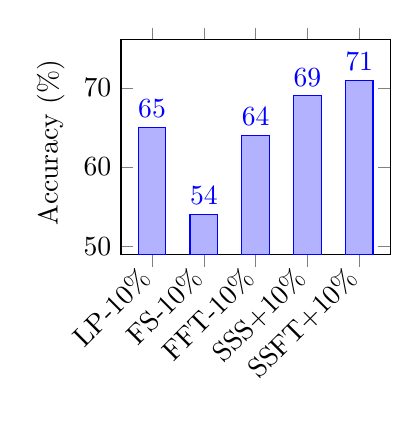
\begin{tikzpicture}
                \begin{axis}
                    [
                    width=5cm,
%                        height=0.4\textwidth,
                    ybar,
%                        bar width=0.2cm,
%                        enlargelimits=0.15,
                    enlarge x limits=0.15,
                    enlarge y limits=0.30,
                    ylabel={\ Accuracy (\%)}, % the ylabel must precede a # symbol.
%                    xlabel={\ Method},
                    symbolic x coords={LP-10, FS-10, FFT-10, SSS+10, SSFT+10}, % these are the specification of coordinates on the x-axis.
                    xtick=data,
                    %            xticklabels={FS\\10\%, FFT\\10\%, SSS\\+10\%, SSFT\\+10\%, FS\\100\%, FFT\\100\%, SSS\\-100\%, SSFT\\-100\%},
                    %            xticklabel style={align=center},
                    xticklabels={LP-10\%, FS-10\%, FFT-10\%, SSS+10\%, SSFT+10\%},
                    xticklabel style={rotate=45,anchor=east},
                    nodes near coords, % this command is used to mention the y-axis points on the top of the particular bar.
                    nodes near coords align={vertical},
                    ]
                    \addplot coordinates { (LP-10, 65) (FS-10, 54) (FFT-10, 64) (SSS+10, 69) (SSFT+10, 71)};

                \end{axis}
            \end{tikzpicture}

            \caption{CIFAR-100}\label{fig:SPARC100}
        \end{subfigure}
        \hfill
        \begin{subfigure}{.33\linewidth}
            \centering

            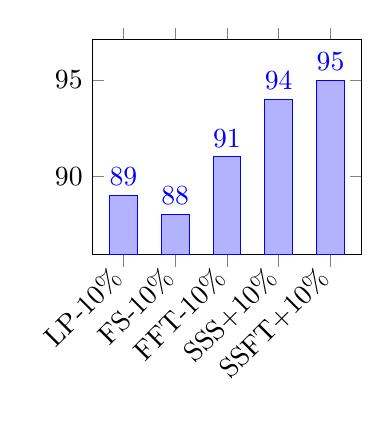
\begin{tikzpicture}
                \begin{axis}
                [
                    width=5cm,
%                        height=0.4\textwidth,
                    ybar,
%                        bar width=0.2cm,
%                        enlargelimits=0.15,
                    enlarge x limits=0.15,
                    enlarge y limits=0.30,
%                    ylabel={\ Accuracy}, % the ylabel must precede a # symbol.
%                    xlabel={\ Method},
                    symbolic x coords={LP-10, FS-10, FFT-10, SSS+10, SSFT+10}, % these are the specification of coordinates on the x-axis.
                    xtick=data,
                %            xticklabels={FS\\10\%, FFT\\10\%, SSS\\+10\%, SSFT\\+10\%, FS\\100\%, FFT\\100\%, SSS\\-100\%, SSFT\\-100\%},
                %            xticklabel style={align=center},
                    xticklabels={ LP-10\%, FS-10\%,FFT-10\%, SSS+10\%, SSFT+10\%},
                    xticklabel style={rotate=45,anchor=east},
                    nodes near coords, % this command is used to mention the y-axis points on the top of the particular bar.
                    nodes near coords align={vertical},
                ]
                    \addplot coordinates { (LP-10, 89) (FS-10, 88) (FFT-10, 91) (SSS+10, 94) (SSFT+10, 95)};

                \end{axis}
            \end{tikzpicture}

            \caption{CIFAR-10}\label{fig:sparC10}
        \end{subfigure}
    \end{figure}

    \begin{figure}
        \caption{ResNet-50 (SWAV), in the 100\% of data case, SSL underperforms by quite a bit on C100. Probably best to just mention this and and put the plot in the appendix, as it is not what we care about.)}
        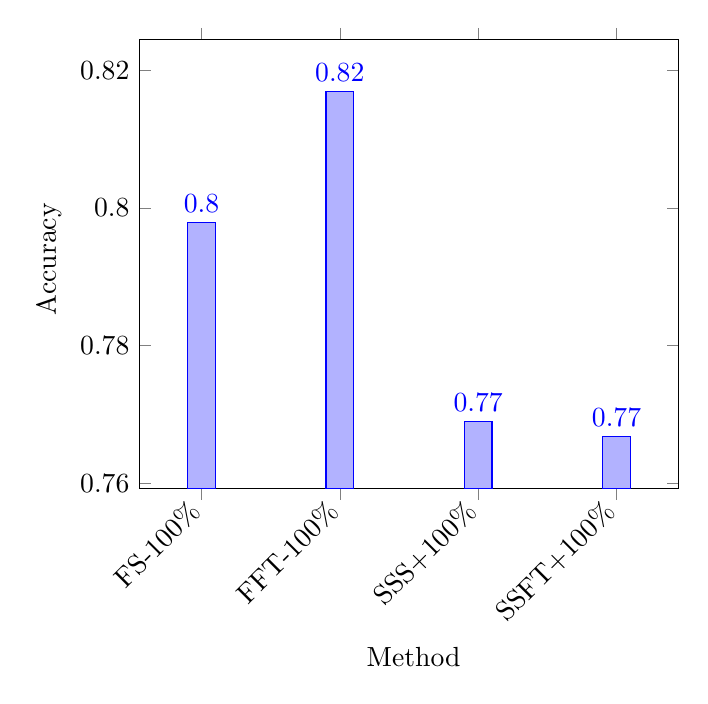
\begin{tikzpicture}

            \begin{axis}
            [
                ybar,
                enlargelimits=0.15,
                ylabel={\ Accuracy}, % the ylabel must precede a # symbol.
                xlabel={\ Method},
                symbolic x coords={FS-100, FFT-100, SSS+100, SSFT+100}, % these are the specification of coordinates on the x-axis.
                xtick=data,
%            xticklabels={FS\\10\%, FFT\\10\%, SSS\\+10\%, SSFT\\+10\%, FS\\100\%, FFT\\100\%, SSS\\-100\%, SSFT\\-100\%},
%            xticklabel style={align=center},
                xticklabels={FS-100\%, FFT-100\%, SSS+100\%, SSFT+100\%},
                xticklabel style={rotate=45,anchor=east},
                nodes near coords, % this command is used to mention the y-axis points on the top of the particular bar.
                nodes near coords align={vertical},
            ]
                \addplot coordinates {(FS-100, 0.7979) (FFT-100, 0.8169) (SSS+100, 0.769) (SSFT+100, 0.7668)};

            \end{axis}
        \end{tikzpicture}
    \end{figure}


    \section{Conclusion}
%%%%%%%%%%%%%%%%%%%%%%%%%%%%%%%%%%%%%%%%%%%%%%%%%%%%%%%%%%%%


    \appendix

    \clearpage


    \section{Appendix}

    \newcommand{\mytableread}[1]{%
        \pgfplotstabletypeset[
            col sep = tab,
            string type,
            string replace*={_}{\textsubscript},
            every head row/.style={before row=\toprule,after row=\midrule},
            every last row/.style={after row=\bottomrule},
        %display columns/0/.style={string type}
        ]
        {#1}
    }

    For each of the models RN18-TiMM\ref{tab:rn18-timm_acc}\ref{tab:rn18-timm_sparsity},
    RN50-PYTORCH,
    RN50-SWAV\ref{tab:rn50-swav_acc}\ref{tab:rn50-swav_sparsity},
    RN50-CLIP,
    T-CLIP.

    \begin{table}[h]
        \captionsetup{aboveskip=5pt,belowskip=5pt}
        \caption{ResNet-18 (TIMM)}

        \begin{subtable}{.60\linewidth}
            \centering
            \mytableread{./plots/part2_accuracy/vertical/part2_rn18-timm_acc.csv}
            \caption{Accuracy}\label{tab:rn18-timm_acc}
        \end{subtable}
        \hfill
        \begin{subtable}{.30\linewidth}
            \centering
            \mytableread{./plots/part2_accuracy/vertical/part2_rn18-timm_sparsity.csv}
            \caption{Sparsity}\label{tab:rn18-timm_sparsity}
        \end{subtable}
    \end{table}

    \begin{table}[h]
        \captionsetup{aboveskip=5pt,belowskip=5pt}
        \caption{ResNet-50 (SWAV)}

        \begin{subtable}{.30\linewidth}
            \centering
            \mytableread{./plots/part2_accuracy/vertical/part2_rn50-swav_acc.csv}
            \caption{Accuracy}\label{tab:rn50-swav_acc}
        \end{subtable}
        \hfill
        \begin{subtable}{.30\linewidth}
            \centering
            \mytableread{./plots/part2_accuracy/vertical/part2_rn50-swav_sparsity.csv}
            \caption{Sparsity}\label{tab:rn50-swav_sparsity}
        \end{subtable}
    \end{table}

    \begin{table}[h]
        \caption{Accuracy KNN}
        \mytableread{./plots/part2_accuracy/vertical/part2_rn18-timm_acc_knn.csv}
    \end{table}

%\begin{table}[h]
%  \caption{IDs}
%  \mytableread{./plots/part2_accuracy/vertical/part2_rn18-timm_ids.csv}
%\end{table}

    \begin{table}[h]
        \caption{Accuracy KNN}
        \mytableread{./plots/part2_accuracy/vertical/part2_rn50-swav_acc_knn.csv}
    \end{table}

    \subsection{Proofs}

    \subsubsection{Translation invariance of threshold and score initialization}\label{proof:translation_invariance}

    \begin{align}
%        \label{eq:threshold}
        m_i^t &= [\theta_i^t > k]
    \end{align}

    where $k$ is the threshold

    \begin{align}
        \theta_i^{t} &= \theta_i^0 - \sum_{\hat t=0}^{t-1} \gamma^{\hat t} g_{i}(\mathcal{M}^{\hat t}, \mathcal{B}^{\hat t})
    \end{align}

    where $g_{i}(\mathcal{M}^{\hat t}, \mathcal{B}^{\hat t})$ is the gradient of the $i$'th weight given the mask $\mathcal{M}^{\hat t}$ and batch $\mathcal{B}^{\hat t}$ (including momentum if enabled)

    \begin{align}
        m_i^0 &= [\theta_i^0 > k] &= [\theta_i^0 + a > k + a] \\
        m_i^{t} &= [\theta_i^0 - \sum_{\hat t=0}^{t-1} \gamma^{\hat t} g_{i}(\mathcal{M}^{\hat t}, \mathcal{B}^{\hat t}) > k] &= [\theta_i^0 + a - \sum_{\hat t=0}^{t-1} \gamma^{\hat t} g_{i}(\mathcal{M}^{\hat t}, \mathcal{B}^{\hat t}) > k + a]\label{eq:recur}
    \end{align}

    For the base case we then have that replacing $\theta_i^0$ with $\theta_i^0 + a$ and $k$ with $k+a$ will not change $m_i^0$ for any $i$, which means the network mask $\mathcal{M}^0$ is also invariant to this change.
    Consequently, $m_i^1$ is also invariant to this change because of eq.~\ref{eq:recur} and because the gradient $g_i(\mathcal{M}^0, \mathcal{B}^0)$ does not change. The same reasoning can be applied recursively to $m_i^2$ and so on. Thus, by induction, translating the initial score and threshold by the same amount will not change any of the network masks during training (under simple sgd without weight decay).

    \subsubsection{Scale invariance of learning rate and score initialization}\label{proof:scale_invariance}

    Equation for sgd with weight decay:

    \begin{align}
        \theta_i^t &= \theta_i^{t-1} - \gamma^t \left( g_i(\mathcal{M}^{t-1}, \mathcal{B}^{t-1}) + \lambda \theta_i^{t-1} \right)
    \end{align}

    Say we replace $\gamma^t$ with $\gamma^t \alpha$, $\theta_i^{t-1}$ with $\theta_i^{t-1} \alpha$ and $\lambda$ with $\frac{\lambda}{\alpha}$ for some $\alpha \in \mathbb{R}^+$, then we get:

    \begin{align}
        \alpha\theta_i^{t-1} - \alpha\gamma^t \left( g_i(\mathcal{M}^{t-1}, \mathcal{B}^{t-1}) + \frac{\lambda}{\alpha} \alpha\theta_i^{t-1} \right) &= \alpha \left(\theta_i^{t-1} - \gamma^t \left( g_i(\mathcal{M}^{t-1}, \mathcal{B}^{t-1}) + \lambda \theta_i^{t-1} \right)\right)\\
        &= \alpha\theta_i^{t}\label{eq:krrrt}
    \end{align}

    Similarly to the previous proof, the initial masks $m_i^0 = [\theta_i^0 > 0]$ are invariant to the scale change $m_i^0 = [\alpha\theta_i^0 > 0]$, so the replacement of $\theta_i^0$ with $\alpha\theta_i^0$, combined with the other replacements, does not change the gradient $g_i(\mathcal{M}^0, \mathcal{B}^0)$. Combined with eq \ref{eq:krrrt}, this means that the updated parameter after the first SGD step is only different in scale when compared to what it would have been without the scale change ($=\alpha\theta_i^t$). Apply this reasoning recursively and it can be seen through induction that the network masks will be the same during training as for the original learning rate, score initialization and weight decay.

    Note that the conclusion still holds when momentum is enabled


%\begin{table}[h]
%  \caption{IDs}
%  \mytableread{./plots/part2_accuracy/vertical/part2_rn50-swav_ids.csv}
%\end{table}

\end{document}